%\subsection{Leksikalsk analyse}
\begin{frame}
  \frametitle{Leksikalsk analyse}

  \begin{itemize}
    \item Lexemes $\rightarrow$ Tokens
    \item Ingen specific syntaks
    \item To klasser: Scanner og Token
      \begin{itemize}
	\item Diverse scan-metoder
	\item (\textbf{Type} tokenType, \textbf{String}
        value, \textbf{int} line, \textbf{int} offset)
      \end{itemize}
      
  \end{itemize}

\end{frame}

%\begin{frame}
%  \frametitle{Leksikalsk analyse} 
  
%  \begin{ebnf}
%    \grule{decimal}{\gter{0} \gor \gter{1} \gor \grange \gor \gter{9}}
%    \grule{lowercase}{\gter{a} \gor \gter{b} \gor \grange \gor \gter{z}}
%    \grule{uppercase}{\gter{A} \gor \gter{B} \gor \grange \gor \gter{Z}}
%    \grule{anycase}{lowercase \gor uppercase}
%    \grule{alphanum}{anycase \gor decimal}
%    \grule{quotebs}{\gtdq \gor \gtbs}
%    \grule{unichar}{\gcomment{any unicode character}}
%    \grule{strchar}{unichar \gex quotebs}
%  \end{ebnf}
%\end{frame}

\begin{frame}
  \frametitle{Leksikalsk analyse}

  \begin{figure}
    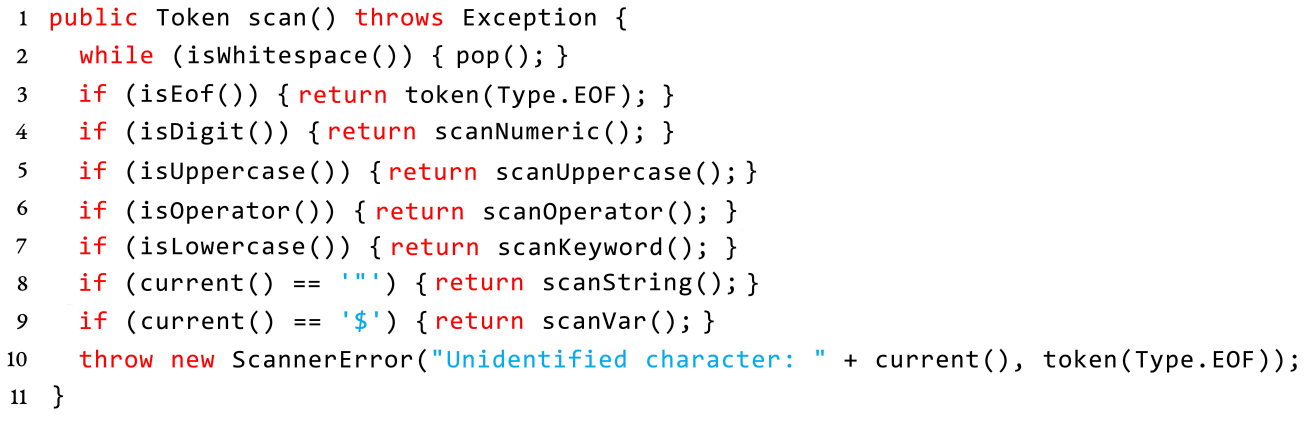
\includegraphics[width=1\linewidth]{billeder/scan-metode}
  \end{figure}

\end{frame}

\begin{frame}
  \frametitle{Leksikalsk analyse}

  \begin{figure}
    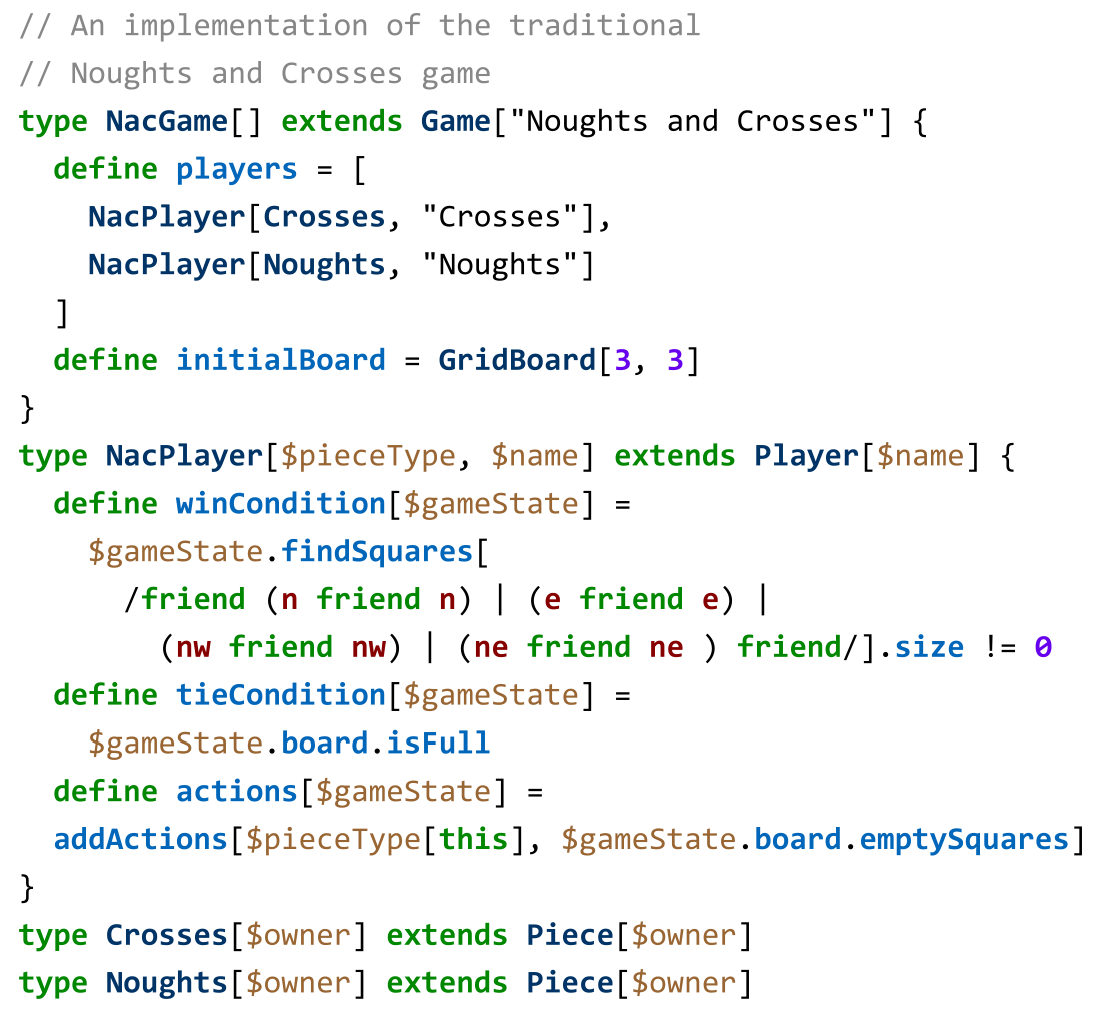
\includegraphics[width=0.6\linewidth]{billeder/krydsogbolle}
  \end{figure}
\end{frame}

